% !TeX encoding = UTF-8
% !TeX spellcheck = en_US
% !TEX root = templateExamSolution.tex
\documentclass[a4paper]{scrartcl}
\usepackage[T1]{fontenc}
%\usepackage[utf8]{inputenc}
\usepackage[english]{babel} \usepackage[bottom=2.5cm,top=2.0cm,left=2.0cm,right=2.0cm]{geometry}
\usepackage{amssymb,amsmath,amsfonts}
\usepackage{lmodern}
\usepackage{graphicx}
\usepackage{csquotes}
\usepackage{booktabs}
\usepackage[dvipsnames]{xcolor}
\definecolor{mygreen}{rgb}{0,0.4,0}
\definecolor{mygray}{rgb}{0.2,0.2,0.2}
\usepackage[numbered,framed]{matlab-prettifier}
\usepackage[backend=biber,style=authoryear]{biblatex}
\addbibresource{templateExamBiblio.bib}

\begin{document}
\title{Computational Macroeconomics\\Midterm Exam}
\author{Willi Mutschler\\Student ID 123\\willi@mutschler.eu}
\date{Version: \today}
\maketitle\thispagestyle{empty}

\newpage
\tableofcontents\thispagestyle{empty}\newpage \setcounter{page}{1}

\section{Exercise 1}\label{sec:introduction}
This is a \LaTeX~template that might be useful for your exam.

\section{Tables}
Table~\ref{tbl:1} is an example of a table.
\begin{table}[h!]
\centering
\begin{tabular}{lcr}
\multicolumn{3}{c}{Calibration}
\\
\toprule
Parameter Name & Variable & Value
\\
\midrule
risk aversion & \(\sigma_C \) & 2
\\
depreciation rate & \(\delta \) & 0.025
\\
growth rate & \(\gamma \) & 1
\\
Frisch elasticity & \(\varphi \) & 1
\\
\bottomrule
\end{tabular}
\caption{This is the caption for the example table.\label{tbl:1}}
\end{table}

\section{Figures}
Table~\ref{fig:1} is an example of a figure.
\begin{figure}[t!]\centering
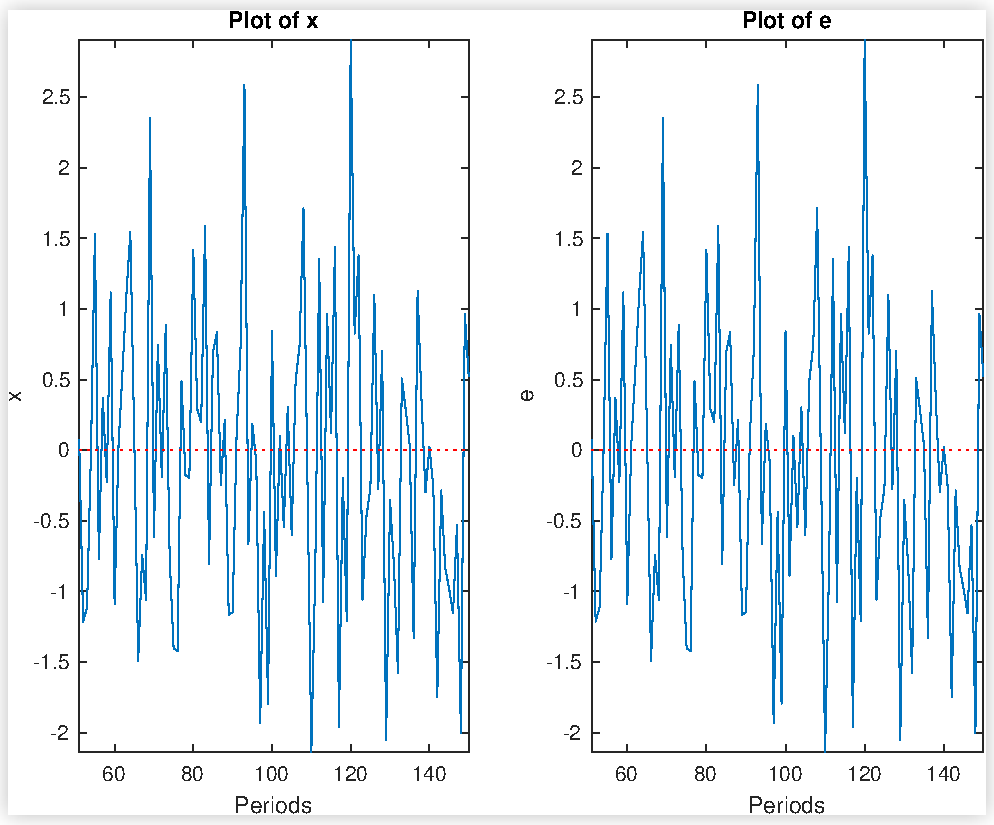
\includegraphics[width=0.75\textwidth]{../../plots/SimulatedTrajectory_x.pdf}
\caption{This is the caption for the example figure.\label{fig:1}}
\end{figure}

\section{Math}
\begin{equation}
e^{\pi i} + 1 = 0\label{eq:euler}
\end{equation}

The beautiful equation~\eqref{eq:euler} is known as the Euler equation. We can also align equations:
\begin{align*}
x &= y & w &= z & a &= b + c
\\
2x &= -y & 3w &= \frac{1}{2}z & -4 + 5x &= 2 + y & w + 2 &= -1 + w & a & = b
\\
ab &= cb
\end{align*}
Inline math works either like this $x_t = A x_{t-1} + \varepsilon_t$ or like this \(\varepsilon_t \overset{iid}\sim \underbrace{N(\underset{3 \times 1}{\boldsymbol{0}},\boldsymbol{\Sigma})}_{\text{normally distributed}}\).
We can also break long lines:
\begin{multline}
p(x) = 3x^6 + 14x^5y + 590x^4y^2 + 19x^3y^3 + 3x^6 + 14x^5y + 590x^4y^2 + 19x^3y^3
\\
- 12x^2y^4 - 12xy^5 + 2y^6 - a^3b^3 - 12x^2y^4 - 12xy^5 + 2y^6 - a^3b^3 \label{eq:long}
\end{multline}
Equation~\eqref{eq:long} is a long equation.
Or group and center lines:
\begin{gather*}
y_t = C x_{t}
\\
x_t = A x_{t-1} + Bu_t
\end{gather*}

\section{Displaying code}
Use \texttt{lstlisting} to display code directly:
\begin{lstlisting}[style = Matlab-editor, basicstyle = \mlttfamily, title = \lstname]
% reshape example
x = reshape(eye(3,3),3*3,1);
% cool solver
dlyap(A,RHS);
\end{lstlisting}
or load it from a file with \texttt{lstinputlisting}
\lstinputlisting[style = Matlab-editor, basicstyle = \mlttfamily, title=\lstname]{../matlab/templateMatlabExample.m}
Note that the pretty formatting for MATLAB is achieved by loading the package \texttt{matlab-prettifier}.

\section{Citations}\label{sec:citations}
Examples how to do citations:
\begin{itemize}
  \item \textcite{Aruoba.Fernandez-Villaverde_2015_ComparisonProgrammingLanguages} compares programming languages in Macroeconomics.
  \item The book \textcite{Heer.Maussner_2024_DynamicGeneralEquilibrium} offers an introduction to numerical methods for solving dynamic general equilibrium models.
  \item Monetary policy is an often studied topic in DSGE models \parencite{Christiano.Trabandt.Walentin_2010_DSGEModelsMonetary}.
\end{itemize}
Now let's print the bibliography.
\newpage
\printbibliography%
\end{document}